El módulo del servidor se encarga de gestionar la lógica de negocio y la comunicación con la base de datos. A continuación, se presenta el diagrama de paquetes del servidor, que muestra la organización de sus componentes y la interacción entre ellos.
\\[1ex]
El servidor está compuesto por los siguientes paquetes:
\begin{itemize}
	\item \textbf{API:} Define la interfaz de comunicación entre el cliente y el servidor, especificando los endpoints disponibles.
	\item \textbf{Rutas:} Maneja la definición y el manejo de las rutas que el servidor expone, asociando cada ruta a su controlador correspondiente.
	\item \textbf{Middlewares:} Aplica funciones intermedias en la cadena de solicitudes HTTP, como autenticación, validación de datos y manejo de errores.
	\item \textbf{Controladores:} Contienen la lógica que maneja las solicitudes del cliente, delegando tareas específicas a los servicios y middlewares.
	\item \textbf{Servicios:} Implementan la lógica de negocio, realizando operaciones complejas y coordinando la interacción entre controladores y modelos.
	\item \textbf{Modelos:} Interactúan con la base de datos, definiendo la estructura de los datos y proporcionando métodos para su manipulación.
\end{itemize}

El diagrama también muestra cómo el cliente se comunica con la API del servidor y cómo el servidor maneja las solicitudes a través de sus componentes hasta llegar a la base de datos y viceversa.

\begin{figure}[H]
	\centering
	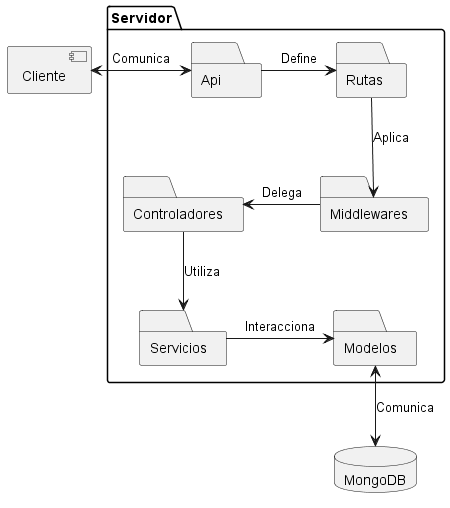
\includegraphics[width=1\linewidth]{6-DiseñoDelSistemaDeInformacion/Modulos/servidor.png}
	\caption{Diagrama de paquetes del Servidor}
\end{figure}